\section{Input length and canvas tuning}
\label{app:input_canvas}

\subsection{Input length}
The input-length sweep repeats the schema block while holding the
extraction target fixed. DG's fitted input slope is approximately
\inputSlopeRatio$\times$ that of dense AR-3B. This demonstrates
input dependence in the tested paths. It does not imply that DG
recomputes all prompt KV state at every denoising step, nor does it
supply an input slope for AR-30B.

\begin{figure}[ht!]
\centering
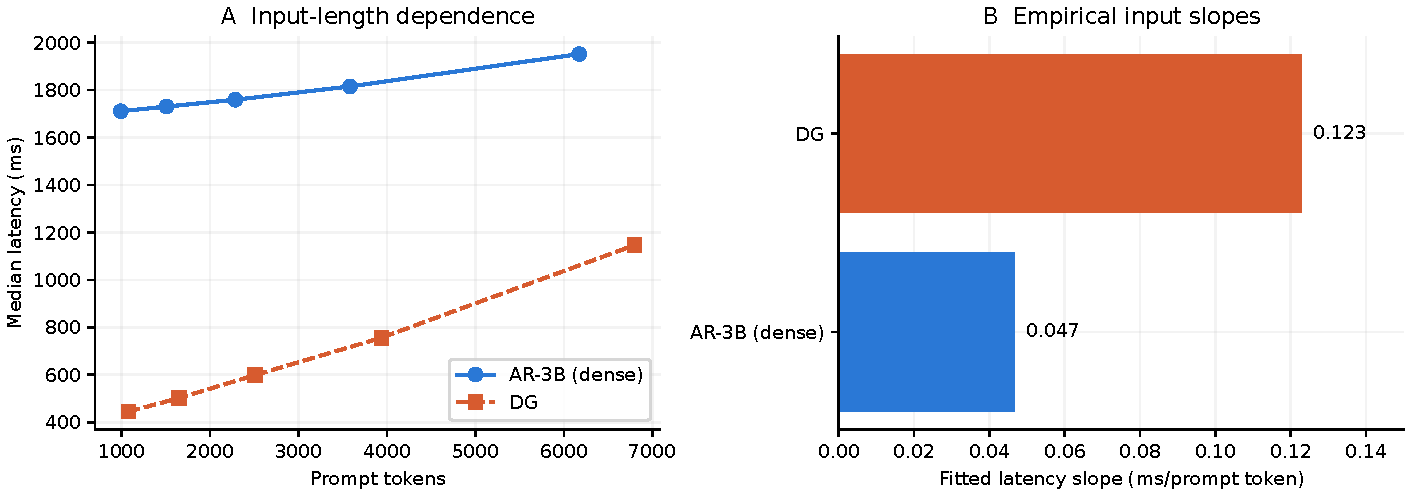
\includegraphics[width=\linewidth]{figures/fig3_input_sweep.pdf}
\caption{Input-length sweep at fixed output budget \canvasLength{}
(BGL, $n{=}100$ per cell; dense AR-3B baseline). Repeating the schema
changes the prompt length and redundancy together. Fitted slopes are
specific to this construction.}
\label{fig:input}
\end{figure}

\subsection{Canvas size and effort}
In the single-parameter sweep, canvas 128 yields median latency
\canvasOneTwentyEightBase\,ms and 9-field F1
\canvasOneTwentyEightFone{}. The joint sweep over canvas sizes
$\{64,128,256,512\}$ and $K\in\{2,4,8,16,32\}$ uses
$n{=}200$ per cell. At $K{=}8$, canvas 128 has observed p50
368\,ms and F1 0.864, compared with 376\,ms and 0.853 for canvas
256. It therefore dominates the reference setting in these two point
estimates. This is an empirical Pareto comparison over the tested grid,
not proof of a global optimum or a statistically established improvement.

Canvas 64 performs worse in the reported setting, but this does not make
it unusable for other output distributions. The reference setting remains
canvas 256, $K{=}8$ for continuity with the principal sweeps. Selecting a
new operating point should include uncertainty, valid-output rates, and
held-out workload evaluation rather than optimization on the same sample.
The joint data are in \texttt{results/issue114\_joint\_sweep.json}.
